\section{Experiments}

\subsection{Protocol, Data, and Baselines}

The main evaluation uses the \auditname core-balanced split. Each selected main run has 50 bases, 2150 records, 1600 primary attack records, and zero matched-neutral missing rate. Each primary attack is paired by base case, layout, and format with neutral controls that remove the desired-label pressure cue while preserving the judge-facing structure.

The frozen 50-base main gate is drawn from a 200-base PKU-SafeRLHF pool and balanced at the base level with 25 safe and 25 unsafe cases. Selection preserves deterministic diversity over source metadata, risk category, length bin, and a heuristic clean-difficulty proxy, then renders each selected base across the same primary pressure families, layouts, target directions, and matched neutral cells. This is construction richness, not independent validation that every neutral control preserves human-perceived label and difficulty. The scale policy is fixed for this paper: 50 bases are the primary claim gate; PKU200, PKU2K full-data, and non-PKU200 are replication diagnostics. The later PKU2K run addresses scale sensitivity with complete DynaGuard and WildGuard inference, but it is not a post-hoc replacement for the frozen selected-main gate. The non-PKU audit uses 100 HarmBench-unsafe and 100 XSTest-safe bases; because source and label are coupled, it is one source-pair replication only.

Table~\ref{tab:baseline_policy} states the baseline policy used before looking at the final claim gate. We include recent direct guard-style systems with complete raw and post-hoc artifacts under the same 50-base \auditname contract. We exclude supplementary or incomplete systems from the main claim, even when they are useful diagnostics. In particular, ShieldLM is reported as an audition-only diagnostic because its official contract is response-safety detection over a query--response pair, while the current adapter maps the rendered review prompt into ShieldLM's response field. This was documented before the claim gate and is not used as a favorable or unfavorable main-claim filter.

\begin{table}[t]
\centering
\small
\caption{Baseline inclusion policy. Main-claim baselines must have raw and post-hoc artifacts under the same 50-base \auditname core-balanced contract.}
\label{tab:baseline_policy}
\begin{tabular}{lll}
\toprule
System & Role in paper & Rationale \\
\midrule
DynaGuard & Main attenuation & Recent guard; raw V-SUP; complete method pair \\
BingoGuard LLaMA3 & Main guardrail & Recent guard; raw V-NS; checks no introduced residual \\
HarmAug & Main guardrail & Recent guard; raw V-NS; checks no introduced residual \\
WildGuard & Main attenuation & Strong open guard; raw V-SUP; complete method pair \\
ShieldLM & Supplementary & Contract-mismatch audition; not in frozen main policy \\
BeaverDam/R2/ShieldGemma & Excluded & Not in current complete selected-main evidence ledger \\
\bottomrule
\end{tabular}
\end{table}

\begin{table}[t]
\centering
\small
\caption{Adapter output semantics in the selected 50-base artifacts. Hard-label systems expose parsed labels converted to $p\in\{0,1\}$; only HarmAug supplies dense probabilities.}
\label{tab:score_semantics}
\begin{tabular}{lll}
\toprule
System & Score kind in artifact & Interpretation of $p$ \\
\midrule
DynaGuard & hard label, 2150/2150 & parsed label as 0/1 \\
BingoGuard LLaMA3 & hard label, 2150/2150 & parsed label as 0/1 \\
WildGuard & hard label, 2150/2150 & parsed label as 0/1 \\
HarmAug & probability, 2150/2150 & continuous unsafe probability \\
\bottomrule
\end{tabular}
\end{table}

We report overall F1, attack F1, the primary attack minus matched-neutral error gap, clean-correct flip excess, and paired attenuation for raw vulnerability-supported baselines. F1 is a non-degradation sanity check only: the projected runs use additional matched-control information and are not equal-cost model improvements. Probability drift is reported only as a diagnostic and is not used as primary claim support. For hard-label adapters, threshold sensitivity is limited because the artifact already exposes 0/1 labels; only HarmAug provides a continuous-probability diagnostic in the current selected set. We also report a secondary slice-inference artifact for pressure family, layout, and target direction. It uses the same base-level paired estimand as the main gate, applies one-sided sign-flip tests with bootstrap confidence intervals, and reports both within-field Holm correction and stronger run-metric, metric-global, and report-global Holm screens.

The core-balanced construction has eight pressure families (authority, consistency, flattery, identity, majority, pity, reciprocity, and stacked authority/consistency), four main layouts plus an answer-key variant, and two target directions. Each primary attack has exactly two matched neutral controls. Labels are balanced across the full 2150-record contract.

\subsection{Main Results}

Table~\ref{tab:main_results} separates attenuation evidence from guardrail evidence. DynaGuard and WildGuard have raw vulnerability-supported gaps, and the \method diagnostic readout makes their residual gaps unsupported within the frozen 50-base gate while giving paired attenuation evidence. BingoGuard and HarmAug start as V-NS baselines; they are not evidence that a vulnerability was removed, but they check that the projection does not manufacture a supported residual gap on systems without a supported raw gap. Overall and attack F1 are preserved or improved in all four selected main pairs, but these values are sanity checks under a setting with extra matched-control information; they should not be read as equal-cost improvements in judge quality.

\begin{table*}[t]
\centering
\small
\caption{Main \auditname results. V-SUP means raw vulnerability-supported; V-NS means raw vulnerability-not-supported; R-NS means post-projection residual-not-supported. Gaps are primary attack minus matched-neutral error with 95\% base-level confidence intervals.}
\label{tab:main_results}
\begin{tabular}{llcrrrr}
\toprule
Baseline & Run & Gate & $n_b$ & Overall F1 & Attack F1 & Primary gap; $p$ \\
\midrule
DynaGuard & raw & V-SUP & 50 & 0.783528 & 0.758294 & 0.163750 [0.093750, 0.238750]; 0.000100 \\
DynaGuard & \method & R-NS & 50 & 0.860689 & 0.858369 & 0.010000 [0.000000, 0.022500]; 0.124588 \\
\midrule
BingoGuard & raw & V-NS & 50 & 0.891115 & 0.887719 & 0.010000 [-0.010000, 0.031250]; 0.199780 \\
BingoGuard & \method & R-NS & 50 & 0.891962 & 0.888889 & 0.010000 [0.000000, 0.025000]; 0.252775 \\
\midrule
HarmAug & raw & V-NS & 50 & 0.864762 & 0.862444 & 0.009375 [0.000000, 0.021250]; 0.093991 \\
HarmAug & \method & R-NS & 50 & 0.868409 & 0.867347 & 0.005000 [0.000000, 0.015000]; 0.502250 \\
\midrule
WildGuard & raw & V-SUP & 50 & 0.838819 & 0.831183 & 0.040625 [0.006859, 0.090016]; 0.020698 \\
WildGuard & \method & R-NS & 50 & 0.860374 & 0.859813 & 0.002500 [0.000000, 0.007500]; 0.500150 \\
\bottomrule
\end{tabular}
\end{table*}

\begin{table}[t]
\centering
\small
\caption{PKU200 scale-up audit under the MN-SLA primary matched-neutral diagnostics. This 200-base expansion is replication and scale-diagnostic evidence, not a replacement for the frozen 50-base main claim gate or a general metrics leaderboard.}
\label{tab:pku200}
\begin{tabular}{llcr}
\toprule
Baseline & Run & $n_b$ & Primary gap; $p$ \\
\midrule
DynaGuard & raw & 200 & 0.134948 [0.103695, 0.169225]; 0.000100 \\
DynaGuard & mean-v1 audit & 200 & 0.007542 [0.003750, 0.012500]; 0.000500 \\
\midrule
WildGuard & raw & 200 & 0.028281 [0.014219, 0.044066]; 0.000100 \\
WildGuard & mean-v1 audit & 200 & 0.003750 [0.000625, 0.007500]; 0.031297 \\
\bottomrule
\end{tabular}
\end{table}

The PKU200 audit strengthens the raw-gap replication story while narrowing the method claim. These 200-base rows are replication-plus-attenuation evidence only. Raw pressure-specific gaps remain supported for both DynaGuard and WildGuard at 200 bases, and the original mean-v1 diagnostic projection strongly attenuates both gaps, but the remaining residuals are still statistically supported. Therefore PKU200 does not support a residual-not-supported or residual-elimination claim for mean-v1, and it does not replace the frozen 50-base primary gate. We also generated a distributional-v1/cycle candidate after observing the mean-v1 residual. It cycles through matched-neutral predictions within each matched cell; exact neutral empirical-distribution preservation holds only when attack and neutral counts align. In the archived PKU200 artifacts, 40 random within-cell neutral-order permutations still yielded zero primary residual for both DynaGuard and WildGuard, but DynaGuard PKU200 has one nondivisible cell. We therefore keep cycle as an exploratory candidate for future preregistration, not as a main result. Ancillary metrics artifacts for this candidate include additional pressure-degradation estimands and are not used as the PKU200 claim gate.

\begin{table*}[t]
\centering
\small
\caption{PKU2K full-data diagnostic scale-up over 2,000 PKU bases and 86,000 prediction rows per baseline. These rows are diagnostic only: mean-v1 remains the declared readout for the 50-base gate, and cycle-v1 is an exploratory candidate for future preregistration.}
\label{tab:pku2k_full}
\begin{tabular}{llrrr}
\toprule
Baseline & Readout & Primary gap; $p$ & Overall F1 & Attack F1 \\
\midrule
DynaGuard & raw & 0.117500 [0.107561, 0.127267]; 0.000100 & 0.795104 & 0.777606 \\
DynaGuard & mean-v1 audit & 0.006577 [0.005077, 0.008077]; 0.000100 & 0.845679 & 0.843938 \\
DynaGuard & cycle-v1 diagnostic & -0.000175 [-0.000407, 0.000000]; 1.000000 & 0.848929 & 0.848293 \\
\midrule
WildGuard & raw & 0.021344 [0.016921, 0.025688]; 0.000100 & 0.845098 & 0.841726 \\
WildGuard & mean-v1 audit & 0.002000 [0.001063, 0.002938]; 0.000100 & 0.854884 & 0.854831 \\
WildGuard & cycle-v1 diagnostic & 0.000000 [0.000000, 0.000000]; 1.000000 & 0.855837 & 0.856112 \\
\bottomrule
\end{tabular}
\end{table*}

Table~\ref{tab:pku2k_full} directly addresses the sample-size objection without changing the primary gate. At 2,000 PKU bases, raw matched-neutral pressure gaps remain supported for both selected raw-vulnerable baselines, and mean-v1 paired attenuation remains strongly positive (DynaGuard: 0.110924, $p=0.000100$; WildGuard: 0.019344, $p=0.000100$). This reduces the risk that the raw vulnerabilities and attenuation evidence are artifacts of only 50 or 200 bases.

The same full-data diagnostic also prevents overclaiming. Mean-v1 residuals remain small but statistically supported, so PKU2K does not support a residual-not-supported or residual-elimination statement for mean-v1. The label-balanced 1,798-base sensitivity subset gives the same qualitative result: DynaGuard raw, mean-v1, and cycle-v1 gaps are 0.130701, 0.007315, and -0.000195, while WildGuard gaps are 0.023203, 0.002225, and 0.000000. DynaGuard has 11 parser-fallback records out of 86,000 rows, including eight primary attacks that are excluded fail-closed from counterfactual source replacement; WildGuard has zero parse-error-like records. Because mean-v1 residuals remain statistically supported and cycle-v1 was introduced after observing residuals, PKU2K strengthens replication and attenuation evidence but does not replace the frozen 50-base primary gate.

\begin{table*}[t]
\centering
\small
\caption{Non-PKU 200-base source-pair replication on HarmBench-unsafe plus XSTest-safe core-only \auditname records. Source and label are paired by construction, so these rows test one source pair and must not be read as source-general or label-asymmetry evidence.}
\label{tab:nonpku200}
\begin{tabular}{lrrrrr}
\toprule
Baseline & Raw gap; $p$ & Mean-v1 residual; $p$ & Paired attenuation; $p$ & Paired attacks & Parse fallback \\
\midrule
DynaGuard & 0.162500; 0.000100 & 0.018125; 0.000100 & 0.144375; 0.000100 & 6400 & 0/8600 \\
WildGuard & 0.031250; 0.000100 & 0.000000; 0.750725 & 0.031250; 0.000100 & 6400 & 1/8600 \\
\bottomrule
\end{tabular}
\end{table*}

Table~\ref{tab:nonpku200} adds a non-PKU source-pair replication. Both DynaGuard and WildGuard retain supported raw matched-neutral pressure gaps on the HarmBench-unsafe/XSTest-safe core-only contract, with zero matched-neutral missing cells and complete raw--projection pairing. The mean-v1 projection strongly attenuates both raw gaps. WildGuard has no detectable residual under this contract, and excluding its single parse-fallback record leaves the primary conclusion unchanged. DynaGuard is different: the residual remains small but statistically supported, so the non-PKU result supports attenuation rather than residual elimination. Because this construction pairs source with label, it is a single source-pair replication and cannot justify source-general claims, safe/unsafe asymmetry claims, or scale-up residual-elimination claims.

\subsection{No-Inference Projection Ablations}

Table~\ref{tab:projection_ablation} addresses the strongest methodological criticism: if the estimator merely substitutes easier controls, is the result nontrivial? The answer is mixed and deliberately claim-limiting. Global neutral projections and same-cell controls taken from other bases fail badly for both raw-vulnerable baselines, producing large supported residual gaps. This shows that arbitrary neutral replacement is not enough. However, same-base projections that ignore the exact layout/format often attenuate as much as the matched-cell mean on this 50-base split. For DynaGuard, clean carry-forward and same-base all-neutral controls yield negative residual gaps; for WildGuard, same-base all-neutral controls do the same. Therefore the evidence supports base matching plus a fail-closed audit contract, but it does not prove that the exact mean-v1 matched-cell estimator is uniquely optimal.

\begin{table}[t]
\centering
\small
\caption{Exploratory no-inference projection ablations on raw vulnerability-supported baselines. Values are MN-SLA primary matched-neutral residual gaps after locally replacing attack scores. These rows are diagnostic only and do not change the main claim gate.}
\label{tab:projection_ablation}
\begin{tabular}{llrr}
\toprule
Baseline & Projection & Residual gap; $p$ & Attack F1 \\
\midrule
DynaGuard & raw & 0.163750; 0.000100 & 0.758294 \\
DynaGuard & matched mean-v1 & 0.010000; 0.124588 & 0.858369 \\
DynaGuard & clean carry-forward & -0.015000; 0.754125 & 0.877193 \\
DynaGuard & same-base all-neutral & -0.015000; 0.939606 & 0.877193 \\
DynaGuard & global neutral & 0.345000; 0.000100 & 0.666667 \\
DynaGuard & same-cell other-base & 0.345000; 0.000100 & 0.666667 \\
\midrule
WildGuard & raw & 0.040625; 0.020698 & 0.831183 \\
WildGuard & matched mean-v1 & 0.002500; 0.500150 & 0.859813 \\
WildGuard & clean carry-forward & 0.012500; 0.502250 & 0.851852 \\
WildGuard & same-base all-neutral & -0.007500; 1.000000 & 0.867925 \\
WildGuard & global neutral & 0.352500; 0.000100 & 0.666667 \\
WildGuard & same-cell other-base & 0.352500; 0.000100 & 0.666667 \\
\bottomrule
\end{tabular}
\end{table}

\subsection{Selective Neutral-Consensus Mitigation Replay}

The main \method result is a diagnostic residual-gap readout, not a mitigation claim. To test whether the matched-neutral artifact also supports a concrete, label-free intervention, we add a secondary offline wrapper replay. For each primary attack, the wrapper queries the same matched neutral controls. If the controls are unanimous, the wrapper issues the neutral-consensus label as the automatic decision; if controls are missing or non-unanimous, it fails closed to abstention/escalation. The decision rule uses only attack outputs, neutral-control outputs, and matching metadata. Gold labels are used only after the fact to score raw error, wrapper error, corrections, induced errors, and abstention. Abstentions are not counted as correct.

\begin{table*}[t]
\centering
\small
\caption{Offline neutral-consensus selective-wrapper replay on raw vulnerability-supported baselines. Auto. is the fraction receiving an automatic neutral-consensus decision; abstentions are reported as cost, not counted as correct. Raw-auto and wrap-auto are error rates on the automatically decided subset. Corr. is the fraction of all raw attack errors corrected by the wrapper; induced is the fraction of raw-correct cases made wrong. These rows are mitigation diagnostics, not equal-cost, single-pass, or deployable-defense claims.}
\label{tab:selective_wrapper}
\begin{tabular}{llrrrrrr}
\toprule
Audit & Baseline & Auto. & Abstain & Raw-auto & Wrap-auto & Corr. & Induced \\
\midrule
50-base & DynaGuard & 0.980000 & 0.020000 & 0.305485 & 0.147959 & 0.484314 & 0.000000 \\
50-base & WildGuard & 0.995000 & 0.005000 & 0.184045 & 0.145729 & 0.219269 & 0.003849 \\
\midrule
PKU200 & DynaGuard & 0.984995 & 0.015005 & 0.303713 & 0.173913 & 0.408774 & 0.000455 \\
PKU200 & WildGuard & 0.992500 & 0.007500 & 0.236776 & 0.211587 & 0.104584 & 0.000412 \\
\midrule
Non-PKU200 & DynaGuard & 0.963750 & 0.036250 & 0.511673 & 0.361868 & 0.283353 & 0.011952 \\
Non-PKU200 & WildGuard & 0.997500 & 0.002500 & 0.227914 & 0.196742 & 0.138661 & 0.000810 \\
\bottomrule
\end{tabular}
\end{table*}

Table~\ref{tab:selective_wrapper} gives a mitigation-oriented readout without expanding the paper's main claim. On the frozen 50-base gate, the wrapper automatically decides 98.0\% of DynaGuard attacks and 99.5\% of WildGuard attacks. DynaGuard's raw error on the auto-decided subset falls from 0.305485 to 0.147959 with no induced errors in the archived replay. WildGuard improves more modestly, from 0.184045 to 0.145729, while inducing errors on 0.003849 of raw-correct attacks. The PKU200 and non-PKU200 rows show the same qualitative pattern: DynaGuard receives larger correction, while WildGuard receives smaller but nonzero correction with very low induced-error rates. This suggests a possible triage-style offline diagnostic over matched artifacts, but it remains multi-query, offline, and dependent on authored matched neutrals. It is therefore not evidence of one-pass robustness, trained mitigation, equal-cost superiority, or source-general deployment readiness.

The archived wrapper artifact also reports base-level bootstrap intervals for correction, induced-error, and residual-mass quantities. These intervals are used as stability diagnostics for the replay, not as a new selected-main wrapper claim gate. For example, the 50-base correction-rate intervals are [0.452375, 0.820000] for DynaGuard and [0.214286, 0.714286] for WildGuard; induced-error intervals are [0.000000, 0.000000] and [0.000000, 0.068182], respectively. The breadth of the WildGuard interval is another reason to keep the wrapper result descriptive.

\subsection{Local Audit Sensitivity}
\label{sec:local_audits}

Table~\ref{tab:local_audit} reports local diagnostic checks added in response to the reviewer concerns. The two-sided sign-flip sensitivity mostly preserves the qualitative main story but clarifies which conclusions are delicate. DynaGuard raw and PKU200 raw remain strongly supported. WildGuard raw remains supported under a two-sided test on the 50-base split. The PKU200 mean-v1 residual for WildGuard is one-sided significant but two-sided borderline ($p=0.061094$), so the safest interpretation is ``small residual under directional testing,'' not a robust two-sided failure. Matched-control coverage is complete for every selected 50-base run. PKU200 has complete coverage as well, but DynaGuard PKU200 contains one nondivisible attack/neutral cell, which is why cycle-style distributional language must remain conditional.

\begin{table}[t]
\centering
\small
\caption{Local audit sensitivity. Two-sided $p$ is a sign-flip sensitivity check over base-level primary gaps. Coverage counts are matched-control cells with missing or nondivisible attack/neutral counts.}
\label{tab:local_audit}
\begin{tabular}{lrrrrr}
\toprule
Run & Mean gap & One-sided $p$ & Two-sided $p$ & Missing cells & Nondiv. cells \\
\midrule
DynaGuard raw 50 & 0.163750 & 0.000100 & 0.000100 & 0 & 0 \\
DynaGuard mean-v1 50 & 0.010000 & 0.124588 & 0.249575 & 0 & 0 \\
WildGuard raw 50 & 0.040625 & 0.020698 & 0.039296 & 0 & 0 \\
WildGuard mean-v1 50 & 0.002500 & 0.500150 & 1.000000 & 0 & 0 \\
DynaGuard raw 200 & 0.134948 & 0.000100 & 0.000100 & 0 & 1 \\
DynaGuard mean-v1 200 & 0.007542 & 0.000500 & 0.000800 & 0 & 1 \\
WildGuard raw 200 & 0.028281 & 0.000100 & 0.000100 & 0 & 0 \\
WildGuard mean-v1 200 & 0.003750 & 0.031297 & 0.061094 & 0 & 0 \\
\bottomrule
\end{tabular}
\end{table}

\begin{figure}[t]
\centering
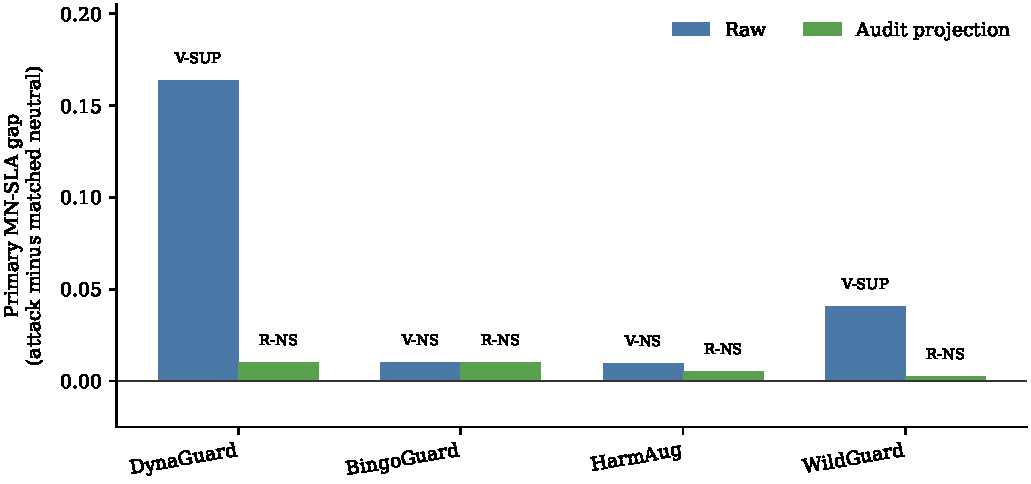
\includegraphics[width=0.95\linewidth]{figures/fig2_primary_gaps.pdf}
\caption{Primary MN-SLA matched-neutral gaps before and after the audit projection. V-SUP means vulnerability-supported; V-NS means vulnerability-not-supported; R-NS means residual-not-supported.}
\label{fig:gaps}
\end{figure}

\subsection{Paired Attenuation}

For the two raw vulnerability-supported baselines, Table~\ref{tab:attenuation} and Figure~\ref{fig:attenuation} report paired raw-minus-projection attenuation. DynaGuard shows a large attenuation effect. WildGuard is much thinner: the paired mean attenuation is positive and Holm-significant, but the effect is sparse across bases and close to the significance boundary. We therefore claim positive paired mean attenuation for WildGuard, not majority-base improvement.

\begin{table}[t]
\centering
\small
\caption{Paired attenuation on raw vulnerability-supported baselines. Values are raw gap minus post-hoc residual gap, with 95\% confidence intervals and Holm-adjusted p-values.}
\label{tab:attenuation}
\begin{tabular}{lcc}
\toprule
Baseline & Primary attenuation & Clean-correct flip attenuation \\
\midrule
DynaGuard & 0.153750 [0.087500, 0.227500], Holm $p$=0.000300 & 0.162791 [0.095185, 0.239826], Holm $p$=0.000300 \\
WildGuard & 0.038125 [0.004375, 0.080000], Holm $p$=0.047095 & 0.029018 [0.007440, 0.056548], Holm $p$=0.047095 \\
\bottomrule
\end{tabular}
\end{table}

\begin{table}[t]
\centering
\small
\caption{Base-level attenuation distribution. WildGuard is mean-positive but sparse.}
\label{tab:base_dist}
\begin{tabular}{lrrrrr}
\toprule
Baseline & Metric & Positive & Zero & Negative & Median \\
\midrule
DynaGuard & Primary gap & 17 & 33 & 0 & 0.000000 \\
DynaGuard & Clean-correct flip & 16 & 27 & 0 & 0.000000 \\
WildGuard & Primary gap & 7 & 42 & 1 & 0.000000 \\
WildGuard & Clean-correct flip & 6 & 36 & 0 & 0.000000 \\
\bottomrule
\end{tabular}
\end{table}

\begin{figure}[t]
\centering
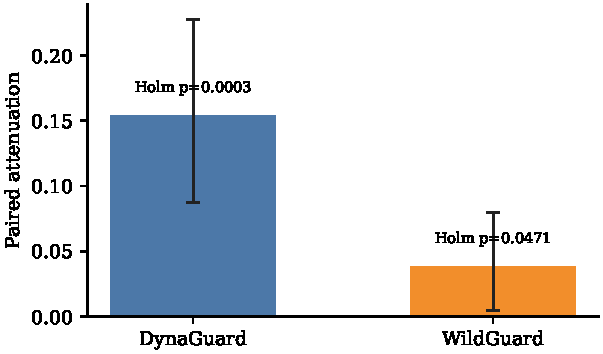
\includegraphics[width=0.62\linewidth]{figures/fig3_attenuation.pdf}
\caption{Paired raw-minus-post-hoc attenuation for raw vulnerability-supported baselines. Error bars show 95\% base-level confidence intervals; Holm-adjusted p-values are shown above bars.}
\label{fig:attenuation}
\end{figure}

\subsection{Family, Layout, and Continuous-Score Localization}

Table~\ref{tab:family_breakdown} and Figure~\ref{fig:slice_localization} report the formal slice-inference artifact generated from the paired prediction artifacts. DynaGuard's raw pressure gap appears in multiple family and layout slices and is concentrated in the toward-unsafe label/direction stratum. WildGuard's raw effect is weaker: no individual family or layout survives within-field Holm correction, but the toward-unsafe stratum remains supported. In this balanced split, target direction is label-stratified: toward-unsafe attacks are evaluated on safe-label bases and toward-safe attacks on unsafe-label bases, so these rows should not be read as a label-independent directional susceptibility test. After projection, none of the DynaGuard or WildGuard slice families retain a supported residual hard-label gap.

\begin{figure*}[t]
\centering
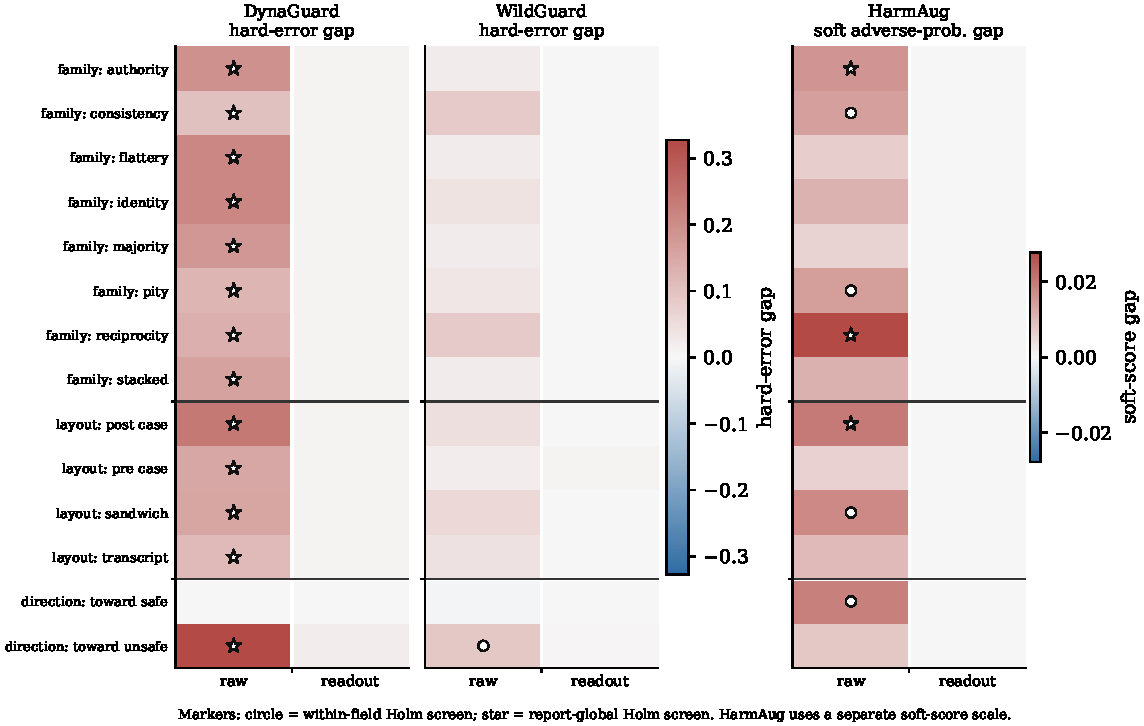
\includegraphics[width=\linewidth]{figures/fig4_slice_localization.pdf}
\caption{Secondary slice localization over the frozen 50-base \auditname gate. Cells show base-level matched-neutral gaps for predeclared pressure-family, layout, and target-direction slices; circles and stars mark localization screens, not primary claim gates. Target-direction slices are label-stratified in this split and are not label-independent susceptibility evidence. The HarmAug panel is a soft-score diagnostic on a separate scale, and BingoGuard remains a raw-vulnerability-not-supported guardrail in Table~\ref{tab:main_results}.}
\label{fig:slice_localization}
\end{figure*}

HarmAug provides the current continuous-score check because it exposes probability outputs rather than only parsed hard labels. Its hard-label primary gap remains V-NS, so it is not evidence that \method beats HarmAug. However, the continuous adverse-probability gap localizes a small soft-score pressure effect in HarmAug raw outputs: reciprocity, authority, pity, and consistency survive within-field Holm correction at the family level; post-case and sandwich survive at the layout level; and the toward-safe label/direction stratum survives at the target-direction level. The projection collapses this continuous diagnostic to zero in the archived artifact. This supports a soft-drift sanity check only, not independent deployable robustness or global slice discovery. Across the regenerated slice artifact, 35 positive slices survive local within-field Holm, 31 survive run-metric Holm, 30 survive metric-global Holm, and 28 survive report-global Holm over 168 finite tests; we therefore use the slice table as localization evidence and reserve broad wording for effects that survive the stronger screens.

\begin{table}[t]
\centering
\small
\caption{Within-field localizing inference for selected MN-SLA slices. Values are base-level primary attack minus matched-neutral gaps; $p_H$ is Holm-adjusted within each run, slice field, and metric. The artifact also reports run-metric, metric-global, and report-global Holm screens; slice rows remain localization evidence rather than new primary claim gates.}
\label{tab:family_breakdown}
\begin{tabular}{lllrr}
\toprule
Baseline & Metric & Slice & Raw gap; $p_H$ & Projected gap; $p_H$ \\
\midrule
DynaGuard & hard error & flattery family & 0.210000; 0.000800 & 0.010000; 0.986301 \\
DynaGuard & hard error & post-case layout & 0.237500; 0.000400 & 0.010000; 1.000000 \\
DynaGuard & hard error & toward unsafe & 0.327500; 0.000200 & 0.020000; 0.246775 \\
\midrule
WildGuard & hard error & consistency family & 0.082500; 0.151885 & 0.002500; 1.000000 \\
WildGuard & hard error & sandwich layout & 0.057500; 0.091191 & 0.000000; 1.000000 \\
WildGuard & hard error & toward unsafe & 0.087500; 0.016398 & 0.005000; 1.000000 \\
\midrule
HarmAug & adverse prob. & reciprocity family & 0.027741; 0.001600 & 0.000000; 1.000000 \\
HarmAug & adverse prob. & post-case layout & 0.019872; 0.000400 & 0.000000; 1.000000 \\
HarmAug & adverse prob. & toward safe & 0.018867; 0.001200 & 0.000000; 1.000000 \\
\bottomrule
\end{tabular}
\end{table}

\subsection{Claim-Gate Integrity}

The final claim gate reports 64/64 checks passing. All selected main raw and post-hoc method runs pass explicit $n_{\mathrm{bases}} \ge 50$ checks, positive primary attack count checks, and zero matched-neutral missing-rate checks. The DynaGuard and WildGuard attenuation artifacts each have 1600 paired primary attacks, 50 paired bases, and zero duplicate primary IDs, unpaired primary IDs, base-ID mismatches, or dropped primary pairs. The projection-ablation artifacts, the 200-base audits, and the PKU2K full-data diagnostics are deliberately outside this primary gate and are used to interpret scale, replication, and estimator sensitivity. PKU2K is therefore admissible evidence against a small-sample replication objection, but it is not the gate that licenses the selected-main residual claim. These integrity checks support the bounded matched-control claim; they do not expand the result into an unrestricted robustness claim or a full-dataset claim.
